\documentclass{article}
\usepackage{graphicx} % Required for inserting images
\usepackage{amsmath}
\usepackage{amssymb}
\usepackage{xcolor}
\usepackage[parfill]{parskip}
\usepackage{bbm}
\usepackage{hyperref}
\usepackage{booktabs}
\usepackage{geometry}
\geometry{margin=1in}
\newcommand{\vl}[1]{\textcolor{orange}{[VL: #1]}}
\newcommand{\eli}[1]{\textcolor{orange}{[Eli: #1]}}
\allowdisplaybreaks

\title{Causal Effect Estimation with Text}
\author{}
\date{}

\begin{document}
	
\maketitle

\section{Problem setting}

Consider a collection of texts (e.g., documents, sentences, utterances) $\mathcal{X}$, with individual texts $X_i \in \mathcal{X}$.
\begin{itemize}
    \item Let $X_i = \{g(X_i), h(X_i)\}$, where $g(X_i)$ is the text attribute of interest (i.e., the \textit{treatment}) and $h(X_i)$ denotes all other properties of the text $X_i$. 
    \item Let $Y_i(X_i) = Y_i(g(X_i), h(X_i))$ denote the potential \textit{response} or \textit{outcome} of respondent $i$ after reading text $X_i$.
    \item For simplicity, assume
    \begin{itemize}
        \item $g(X_i) \in \{0, 1\}$ $\forall$ $X_i \in \mathcal{X}$.
        \item Each respondent reads only one text. That is, respondent $i$ reads only $X_i$.
    \end{itemize}
\end{itemize}

We are interested in knowing the effect of the text attribute $g(X)$ on the response $Y$. Using the standard causal notation, the \textbf{estimand} $\tau^*$ for the effect of $g(X)$ on $Y$ is given by
\begin{align*}
    \tau^* &= \mathbb{E}_X[Y_i(g(X_i)=1)] - \mathbb{E}_X[Y_i(g(X_i)=0)] \\
    &= \boxed{\sum_{b \in \mathcal{B}} \Big[ \mathbb{E}[Y_i(g(X_i)=1, h(X_i)=b)] - \mathbb{E}[Y_i(g(X_i)=0, h(X_i)=b] \Big]P(h(X_i)=b)}
\end{align*}

Using stochastic notation, we can write $\tau^*$ more simply.
\begin{itemize}
    \item Let $P_{1 g,h}(X)$ denote a distribution such that $g(X)=1$ and $h(X) \sim P^*$, where $P^*$ is some arbitrary probability distribution.
    \item Let $P_{0 g,h}(X)$ denote a distribution such that $g(X)=0$ and $h(X) \sim P^*$.
    \item Let the quantity $\mu(P)$ be defined as follows:
    \begin{align*}
        \mu(P) &= E_{X_i \sim P_{g,h}}[Y_i(X_i)] \\
        &= \frac{1}{N} \sum_{i=1}^N Y_i(X_i)P_{g,h}(X_i)
    \end{align*}
\end{itemize}

This allows us to express $\tau^*$ as
\begin{equation*}
    \boxed{\tau^* = \mu(P_1)-\mu(P_0)}
\end{equation*}

\section{Estimator}

\subsection{Data setting}

Suppose we have some data collected from a randomized trial, in which subjects $i \in [N]$ are shown various texts randomized over $g(X)$ and $h(X)$. These texts are constructed from individual components in a generative way. 
\begin{itemize}
    \item That is, to construct a text where $g(X)=1$, the text may include one of several selected sentences that are chosen to correspond to $g(X)=1$.
    \item Likewise, for various attributes comprising $h(X)=(h_1(X), h_2(X), h_3(X), \dots)$, there may be several candidate texts that correspond to $h_1(X)=1$, several candidate texts that correspond to $h_2(X)=0$, and so on.
\end{itemize}

While we are guaranteed to be able to obtain an unbiased effect estimate for $g(X)$ from this trial (e.g., using the plug-in estimator), the estimate corresponds only to the effect of $g(X)$ \textit{in this specific text setting}.\footnote{``Vignette experiments only provide a local treatment effect. Extrapolating from this local treatment effect to the population of relevant texts requires the strong assumption that the many possible ways of delivering
the latent treatment do not interact with the latent treatment, causing its effect on the outcome to change.'' \cite{fong2021causal}} The type of text setting constructed in this trial is fairly artificial, and we believe that the effect may be different depending on the text setting. It is important, for example, to know if this effect still holds in natural text settings.

Therefore, we are interested in knowing the effect of $g(X)$ under text distributions that are different from the initial text distribution. Again, some notation:

\begin{itemize}
    \item Let $P^R_{g,h} = P^R$ denote the \textit{randomization distribution}, or the distribution of texts as constructed in the randomized trial.
    \item Let $P^T_{g,h} = P^T$ denote the \textit{target distribution}, or the text distribution of interest.
    \item Let $\mathbb{P}(A) = \int_A P(X) dx$.
    \item Using the Radon-Nikodym derivative for change of measure (see Section \ref{sec:change_of_measure}), we can write $P^T$ in terms of $P^R$ as
    \begin{equation*}
        P^T(X) = \frac{d\mathbb{P}^T}{d\mathbb{P}^R}(X)P^R(X)
    \end{equation*}
    \begin{itemize}
        \item We require \href{https://en.wikipedia.org/wiki/Absolute_continuity#Absolute_continuity_of_measures}{absolute continuity} of $\mathbb{P}^T$ with respect to  $\mathbb{P}^R$, such that $P^R(X) = 0 \Rightarrow P^R(X) = 0$.
    \end{itemize}
    \item Now, let $(X_i,Y_i(X_i))_{i=1}^n \sim P^R$ correspond to \textit{observed} pairs of features and outcomes sampled from the randomization distribution $P^R$.
\end{itemize}

\subsection{Horvitz-Thompson estimator}

To define our effect estimate in terms of our target distribution $P^T$, we propose using the ratio between $P^T$ and $P^R$ as importance weights in an Horvitz-Thompson estimator. Using the change of measure for $P^T(X)$ we defined previously, this gives us 
% \vl{Do we need to normalize by $\frac{1}{\sum_{i=1}^n \hat{P}^T(X_i)}$ in the first line?}
\begin{align*}
    \hat{\mu}(P^T) &= \frac{1}{n} \sum_{i=1}^n \frac{\hat{P}^T(X_i)}{P^R(X_i)}Y_i(X_i) \\
    &= \frac{1}{n} \sum_{i=1}^n \frac{\hat{d \mathbb{P}^T}}{d \mathbb{P}^R}(X_i)\frac{P^R(X_i)}{P^R(X_i)} Y_i(X_i) \\
    &=\boxed{\frac{1}{n} \sum_{i=1}^n \frac{\hat{d \mathbb{P}^T}}{d \mathbb{P}^R}(X_i)Y_i(X_i)}
\end{align*}

We can show that $\hat{\mu}(P^T)$ is an unbiased estimator for $\mu(P^T)$:
\begin{align*}
    \mathbb{E}[\hat{\mu}(P)] &= \mathbb{E}_{X \sim P^R}[\hat{\mu}(P)] \\
    &= \mathbb{E}\left[\frac{1}{n} \sum_{i=1}^n \frac{\hat{d \mathbb{P}^T}}{d \mathbb{P}^R}(X_i)Y_i(X_i)\right] \\
    &=\frac{1}{n}\sum_{i=1}^n \mathbb{E}_{X \sim P^R}\left[\frac{\hat{d \mathbb{P}^T}}{d \mathbb{P}^R}(X_i)Y_i(X_i)\right] \\
    &= \mathbb{E}_{X \sim P^R}\left[\frac{\hat{d \mathbb{P}^T}}{d \mathbb{P}^R}(X_i)Y_i(X_i)\right] \\
    &=\mathbb{E}_{X \sim P^T}[Y_i(X_i)] \\
    &= \mu(P^T)
\end{align*}

Finally, letting $\mathcal{X}$ be the space of all texts, the variance of the estimator is given by:
\begin{align*}
    \text{Var}[\hat{\mu}(P)] &= \text{Var}_X\left[\frac{1}{n} \sum_{i=1}^n \frac{\hat{d \mathbb{P}^T}}{d \mathbb{P}^R}(X_i)Y_i(X_i)\right] \\
    &= \text{Cov}_X\left[\frac{1}{n} \sum_{i=1}^n \frac{\hat{d \mathbb{P}^T}}{d \mathbb{P}^R}(X_i)Y_i(X_i), \frac{1}{n} \sum_{j=1}^n \frac{\hat{d \mathbb{P}^T}}{d \mathbb{P}^R}(X_j)Y_j(X_j)\right] \\
    &= \frac{1}{n^2}\sum_{i=1}^n \sum_{j=1}^n \text{Cov}_X\left[\frac{\hat{d \mathbb{P}^T}}{d \mathbb{P}^R}(X_i)Y_i(X_i), \frac{\hat{d \mathbb{P}^T}}{d \mathbb{P}^R}(X_j)Y_j(X_j)\right] \\
    &= \frac{1}{n^2}\sum_{i=1}^n \sum_{j=1}^n \text{Cov}_X\left[\sum_{x \in \mathcal{X}}\frac{\hat{d \mathbb{P}^T}}{d \mathbb{P}^R}(X_i)Y_i(X_i)\mathbbm{1}\{X_i = x\}, \sum_{x' \in \mathcal{X}}\frac{\hat{d \mathbb{P}^T}}{d \mathbb{P}^R}(X_j)Y_j(X_j)\mathbbm{1}\{X_j=x'\}\right] \\
    &= \frac{1}{n^2}\sum_{i=1}^n \sum_{j=1}^n \text{Cov}_X\left[\int_x\frac{\hat{d \mathbb{P}^T}}{d \mathbb{P}^R}(x)Y_i(x)\mathbbm{1}\{X_i = x\}d\mathbb{P}^R(x), \int_{x'}\frac{\hat{d \mathbb{P}^T}}{d \mathbb{P}^R}(x')Y_j(x')\mathbbm{1}\{X_j=x'\}d\mathbb{P}^R(x')\right] \\
    &= \frac{1}{n^2} \sum_{i=1}^n \sum_{j=1}^n \int_x \int_{x'} \frac{d \mathbb{P}^T}{d \mathbb{P}^R}(x)\frac{d \mathbb{P}^T}{d \mathbb{P}^R}(x')Y_i(x)Y_j(x') \text{Cov})_X[\mathbbm{1}\{X_i=x\}, \mathbbm{1}\{X_i=x'\}]d\mathbb{P}^R(x)d\mathbb{P}^R(x') \\
    &= \frac{1}{n^2} \sum_{i,j \in [n]} \iint_{x, x'} \frac{d \mathbb{P}^T}{d \mathbb{P}^R}(x)\frac{d \mathbb{P}^T}{d \mathbb{P}^R}(x')Y_i(x)Y_j(x') \text{Cov}_X[\mathbbm{1}\{X_i=x\}, \mathbbm{1}\{X_i=x'\}]d\mathbb{P}^R(x)d\mathbb{P}^R(x') \\
    &= \frac{1}{n^2} \sum_{i,j \in [n]} \iint_{x, x'} \frac{d \mathbb{P}^T}{d \mathbb{P}^R}(x)\frac{d \mathbb{P}^T}{d \mathbb{P}^R}(x')Y_i(x)Y_j(x') (P^R(x,x') - P^R(x)P^R(x'))d\mathbb{P}^R(x)d\mathbb{P}^R(x')
\end{align*}
\eli{I think this generally gets to the right place, but e.g. the inner term in some of those covariances should be $\int_x\frac{\hat{d \mathbb{P}^T}}{d \mathbb{P}^R}(x)Y_i(x)\mathbbm{1}\{X_i = x\}d\mathbb{P}^R(x)$, so that only $\mathbbm{1}\{X_i = x\}d\mathbb{P}^R(x)$ is random}
where the last equality follows from
\begin{align*}
    \text{Cov}[\mathbbm{1}\{X_i=x\},\mathbbm{1}\{X_j=x'\}] &=\mathbb{E}_X[\mathbbm{1}\{X_i=x\}\mathbbm{1}\{X_j=x'\}] - \mathbb{E}_X[\mathbbm{1}\{X_i=x\}]\mathbb{E}_X[\mathbbm{1}\{X_j=x'\}] \\
    &= P^R(x,x') - P^R(x)P^R(x')
\end{align*}

With the central limit theorem (CLT), we establish asymptotic normality:
\begin{equation*}
    \frac{\hat{\mu}(P) - \mu(P)}{\sqrt{\text{Var}[\hat{\mu}(P)]}}\rightarrow N(0,1)
\end{equation*}

which we can use to estimate confidence intervals using the following unbiased estimate for the variance.
\begin{equation*}
    \widehat{\text{Var}}[\hat{\mu}(P)] = \frac{1}{n^2} \sum_{i,j \in [n]} \frac{\hat{d \mathbb{P}^T}}{d \mathbb{P}^R}(X_i)\frac{\hat{d \mathbb{P}^T}}{d \mathbb{P}^R}(X_j)Y_i(X_i)Y_j(X_j)\frac{P^R(X_i,X_j) - P^R(X_i)P^R(X_j)}{P^R(X_i,X_j)}
\end{equation*}

\vl{The last term of the variance is 0 unless $i=j$, in which case it becomes $$\frac{P^R(X_i,X_i)-P^R(X_i)P^R(X_j)}{P^R(X_i,X_i)} = \frac{P^R(X_i)-P^R(X_i)P^R(X_j)}{P^R(X_i)} = 1-P^R(X_j)$$}

\vl{QUESTION: Do we compute variance estimates separately for $\hat{\mu}(P_1)$ and $\hat{\mu}(P_1)$, then compute $$\widehat{\text{Var}}(\hat{\tau})=\frac{\widehat{\text{Var}}[\hat{\mu}(P_1)]}{n^2P(g(X)=1)^2} + \frac{\widehat{\text{Var}}[\hat{\mu}(P_0)]}{n^2P(g(X)=0)^2}$$ Or do we use this variance estimate over the whole sample to directly get $\widehat{\text{Var}}(\hat{\tau})$?
ANSWER: In the finite-sample setting, adding the variance estimates is fine. In the non-finite-sample setting, the variance estimation is more involved.}

\section{Empirical estimation}
\subsection{Estimating $\hat{P}^T$ from the data}

\vl{QUESTION: Should we ever use the full randomization corpus (i.e., all possible 2- or 3-attribute permutations of candidate sentences from the HK study) as $P^R$, or do we always consider $P^R$ to be the sample (i.e., the data for which we have measured outcomes)? This is relevant because the distributions are not the same---the reason being that there are different numbers of candidate sentences for each text attribute, so a full set of permutations is not uniform over the confounding attributes. 
ANSWER: Instead of getting all possible permutations, get the full randomization distribution by just sampling a large number of texts according to the way Fong \& Grimmer sampled theirs. That is, first sample attributes, then sample sentences from those attributes.}

\vl{As a related question, should the distribution of number of sentences per text in $P^T$ follow sample $P^R$ or full-corpus $P^R$?}

Our estimator has one primary nuisance parameter, $\frac{\hat{d\mathbb{P}^T}(X)}{d\mathbb{P}^R(X)}$ (or $\hat{P}^T(X)$, depending on the version of the estimator we want to use). We propose several approaches for estimating this quantity.

\vl{QUESTION: Is sample splitting necessary when learning the nuisance parameter? For now, I have split off a very small sample (10\% of the data) for training the classifier.
ANSWER: Maybe?}

\subsubsection{Classification}
\label{sec:classification}

We notice that we can rewrite $\frac{d\mathbb{P}^T}{d\mathbb{P}^R}$. Let $C$ denote the distribution (or corpus) from which a text is drawn, where $C=T$ denotes that it is drawn from $P^T$ and $C=R$ denotes that it is drawn from $P^R$. Then
\begin{equation*}
    \begin{split}
        &\frac{d\mathbb{P}^T}{d\mathbb{P}^R}(X) = \frac{P(C=T|X)}{P(C=T)}\frac{P(C=R)}{P(C=R|X)}\\
        \Rightarrow &\frac{\hat{d\mathbb{P}^T}}{d\mathbb{P}^R}(X) = \frac{\hat{P}(C=T|X)}{P(C=T)}\frac{P(C=R)}{\hat{P}(C=R|X)}
    \end{split}
\end{equation*}

where estimation of $\hat{P}(C=T|X)$ and $\hat{P}(C=R|X)$ is straightforward---we can train a binary classifier $M_\theta: \mathcal{X} \rightarrow \{0,1\}$ to predict if a text $X$ came from $T$ or $R$---and $P(C=R)$ and $P(C=T)$ are their sample proportions over the entire body of text.

We have several options for our binary classifier:
\begin{itemize}
    \item A model that takes ``interpretable'' language features as input (e.g., bag-of-words, lexicon, SenteCon). We train a ``simple'' classifier over these features (e.g., logistic regression, SVM).
    \item A deep language model that takes raw text as input. We can either use a pre-trained model, or we can fine-tune the pre-trained model to differentiate between text examples from $P^T$ and text examples from $P^R$.
    \item \vl{Since texts from $P^R$ are artificial, the classification task might be very easy, so $\hat{P}(C=T|X)$ and $\hat{P}(C=R|X)$ may be very close to either 0 or 1. Instead of training a discriminative classifier, we could have two generative models, one for $P^R$ and one for $P^T$. Then given an $X$, which model is more likely? This could help with the overconfidence of the discriminative classifier.}
\end{itemize}

\subsubsection{Language modeling}
\label{sec:language_modeling}

Language models like transformers are capable of directly computing the probability of a sentence (see Section \ref{sec:huggingface_sentence_probs}), even if the model has never seen the sentence before. This probability is based on the text distribution used to train the model. Since the state-of-the-art large language models (LLMs) are pre-trained on extremely large corpora that approximate the entirety of the English language, we must further fine-tune before we can use them to compute sentence probabilities for $P^T$.

LLMs are often trained using masked language modeling (MLM), where for each training sentence, certain words are randomly masked, and the model must predict them. However, it is important to note that token and sentence probabilities from language models trained with MLM are not statistically or linguistically meaningful (this was actually \href{https://github.com/google-research/bert/issues/35}{confirmed} by Jacob Devlin when BERT was released). The token probabilities returned by the model are the probability of the masked token \textit{at a specific position}, \textit{given the rest of the unmasked tokens in the sentence}, rather than the probability of the token \textit{given the preceding tokens in the sentence}. 

Instead, to estimate meaningful sentence probabilities directly, \textit{autoregressive language models}, which are trained on causal language modeling\footnote{There's nothing causal about causal language modeling; it's just a naming convention.} (CLM)/text generation/next-word-prediction tasks, may be used. These include ``shallow'' language models like n-gram language models, as well as autoregressive LLMs like GPT-2, TransformerXL, and Reformer (a partial list of autoregressive LLMs implemented by HuggingFace can be found \href{https://web.archive.org/web/20230125132319/https://huggingface.co/docs/transformers/model_summary#autoregressive-models}{here}).

We can encourage an autoregressive language model $M_\theta$ to learn $P^T$ by fine-tuning it on text examples from $P^T$ using a CLM task. For a practical example of CLM, see \href{https://huggingface.co/docs/transformers/tasks/language_modeling}{this example from HuggingFace}.

% \begin{itemize}
%     \item We draw text examples from $P^T$. For each sentence, certain words are masked, and $M_\theta$ learns to predict them.
%     \item Causal language modeling (CLM)/text generation: Again, we drawn text samples from $P^T$. For each sentence, starting from the first word, $M_\theta$ learns to predict the next word.
%     \item Style transfer: Given a text example drawn from $P^R$, $M_\theta$ reproduces that same text example ``in the style of'' $P^T$. This task requires $M_\theta$ to be a sequence-to-sequence language model, like BART \cite{lewis2020bart}, and for best results, parallel text examples from $P^R$ and $P^T$ should be available.
% \end{itemize}

% For a practical example of MLM and CLM, see \href{https://huggingface.co/docs/transformers/tasks/language_modeling}{this example from HuggingFace}. For some ideas on how to fine-tune BART on a style transfer task, see \href{https://blog.fastforwardlabs.com/2022/05/05/neutralizing-subjectivity-bias-with-huggingface-transformers.html}{this blog post} and \cite{lai2021bart}.

\vl{Because texts from $P^R$ are very artificial (especially the sequences of sentences), it is possible that $P^T$ of those texts will be very low, perhaps more than they should be. $P^T$ of individual sentences may not be that low, but the overall construction will have low probability. Is this a problem? Maybe we should compute $P^T(\text{sentence 1})P^T(\text{sentence 2})P^T(\text{sentence 3})$ instead of $P^T(\text{sentence 1, sentence 2, sentence 3})$...}

\vl{QUESTION: If you fine-tune an LM, how do you guarantee that it's learned enough of $P^T$ and forgotten enough of its original training domain? Also, how do you guarantee that it moves away from $P^R$?
ANSWER: One potential solution is to use a shallow language model and train it \textit{only} on $P^T$, which ensures that the resulting sentence probabilities are defined only over $P^T$.}

\subsection{Estimating $\hat{\mu}(P)$ from the data}

We estimate the overall quantity of interest $\hat{\tau}$ through the following procedure. Suppose we have samples $(X_i,Y_i)_{i=1}^n \sim P^R$. In our experiments, these samples are from \cite{fong2021causal}. The authors conduct a randomized study on the effects of a text attribute $g(X)$ on an outcome $Y$ in a constructed text setting, which we consider to be distributed $P^R$.

\begin{enumerate}
    \item Sample examples from $P^T$. Train $M_\theta$ on these examples to be able to obtain $\frac{\hat{d \mathbb{P}^T}}{d \mathbb{P}^R}(X_i)$ or $\hat{P}^T(X_i)$ $\forall$ $i \in [n]$.
    \begin{itemize}
        \item[--] In our experiments, these examples from $P^T$ constitute 2-7 sentence chunks drawn from the U.S. Congressional speeches on the Hong Kong protests. We consider these to be the ``natural language counterparts'' of the examples from $P^R$.
    \end{itemize}
    \item (If using $P^T$) $P^R(X_i)$ should be known from the design of the randomized study. In the worst case, it can be computed empirically from sample proportions.
    \item Split $(X_i,Y_i)$ according to samples where $g(X_i)=1$ and where $g(X_i)=0$. Call these data splits $D_1$ and $D_0$, respectively.
    \item Compute
    \begin{equation*}
        \begin{split}
            \hat{\tau} &= \hat{\mu}(P_1) - \hat{\mu}(P_0) \\
            &= \frac{1}{nP(g(X)=1)} \sum_{j \in D_1} \frac{\hat{d \mathbb{P}^T}}{d \mathbb{P}^R}(X_j)Y_j - \frac{1}{nP(g(X)=0)} \sum_{k \in D_0} \frac{\hat{d \mathbb{P}^T}}{d \mathbb{P}^R}(X_k)Y_k \\
            &= \frac{1}{nP(g(X)=1)} \sum_{j \in D_1} \frac{\hat{P}(C=T|X_j)}{P(C=T)}\frac{P(C=R)}{\hat{P}(C=R|X_j)}Y_j - \frac{1}{nP(g(X)=0)} \sum_{k \in D_0} \frac{\hat{P}(C=T|X_k)}{P(C=T)}\frac{P(C=R)}{\hat{P}(C=R|X_k)}Y_k
        \end{split}
    \end{equation*}
    or alternatively (to ensure that the absolute continuity condition holds, we restrict $P^T$ with respect to the support of the randomization distribution, such that $P^T(X) = \frac{P^T(\tilde{X})\mathbbm{1}\{\tilde{X} \in C^R\}}{\sum_{i=1}^n P^T(X_i)}$)
    \begin{equation*}
        \begin{split}
            \hat{\tau} &= \hat{\mu}(P_1) - \hat{\mu}(P_0) \\
            &= \frac{1}{n P(g(X)=1)} \sum_{j \in D_1} \frac{\hat{P}^T(X_j)}{P^R(X_j)\sum_{i=1}^n \hat{P}^T(X_i)}Y_j - \frac{1}{nP(g(X)=0)} \sum_{k \in D_0} \frac{\hat{P}^T(X_k)}{P^R(X_k)\sum_{i=1}^n \hat{P}^T(X_i)}Y_k
        \end{split}
    \end{equation*}
    % \vl{Is the normalization just to ensure that $\hat{P}^T$ sums to 1 over $X_i \sim P^R$?}
    
    Note that $P(g(X)=1)$ and $P(g(X)=0)$ are defined over the entire randomization corpus (i.e., every possible permutation of the statements/linguistic attributes in the HK study), prior to sampling. In practical terms, this means they are computed from the  proportions of the randomization corpus, rather than the  proportions of the sampled data (i.e., the data for which we have measured outcomes).
    \item In practice, to maintain the stability of the weights (which can be very small), we use the \href{https://cran.r-project.org/web/packages/sampling/vignettes/HT_Hajek_estimators.pdf}{Hajek estimator} instead of the Horvitz-Thompson estimator. With the Hajek estimator, the importance weights are normalized by the \textit{average} importance weight, which yields the following estimators:
    \begin{equation*}
        \hat{\tau} = \frac{1}{|D_1|} \sum_{j \in D_1} \hat{\gamma}_j Y_j - \frac{1}{|D_0|} \sum_{k \in D_0} \hat{\gamma}_k Y_k
    \end{equation*}
    
    \begin{equation*}
        \widehat{\text{Var}}[\hat{\mu}(P_1)] = \frac{1}{|D_1|^2} \sum_{i,j \in D_1} \hat{\gamma}_i \hat{\gamma}_j (Y_i-\bar{Y}_{D_1})(Y_j-\bar{Y}_{D_1}) \frac{P^R(X_i,X_j)-P^R(X_i)P^R(X_j)}{P^R(X_i,X_j)}
    \end{equation*}
    
    \begin{equation*}
        \widehat{\text{Var}}[\hat{\mu}(P_0)] = \frac{1}{|D_0|^2} \sum_{i,j \in D_0} \hat{\gamma}_i \hat{\gamma}_j (Y_i-\bar{Y}_{D_0})(Y_j-\bar{Y}_{D_0}) \frac{P^R(X_i,X_j)-P^R(X_i)P^R(X_j)}{P^R(X_i,X_j)}
    \end{equation*}

    \vl{Not totally sure about this, but I thought we would have to subtract out the mean $Y$ so that the variance doesn't blow up with large $Y$?}
    
    \begin{equation*}
        \widehat{\text{Var}}[\hat{\tau}] = \widehat{\text{Var}}[\hat{\mu}(P_1)] + \widehat{\text{Var}}[\hat{\mu}(P_0)]
    \end{equation*}
    
    where for the classification approach,
    \begin{equation*}
        \hat{\gamma}_j = \frac{\hat{d \mathbb{P}^T}}{d \mathbb{P}^R}(X_j) \Bigg/ \left(\frac{1}{|D|} \sum_{j \in D} \frac{\hat{d \mathbb{P}^T}}{d \mathbb{P}^R}(X_j)\right)
    \end{equation*}
    and for the language modeling approach,
    \begin{equation*}
        \hat{\gamma}_j = \frac{\hat{P}^T(X_j)}{P^R(X_j)\sum_{i=1}^n \hat{P}^T(X_i)} \Bigg/ \left(\frac{1}{|D|} \sum_{j \in D} \frac{\hat{P}^T(X_j)}{P^R(X_j)\sum_{i=1}^n \hat{P}^T(X_i)} \right)
    \end{equation*}
\end{enumerate}

% \vl{Is there any reason Fong \& Grimmer used linear regression to estimate the effects instead of difference-in-means? I also implemented the option of LR on weight-adjusted $Y_i$s, but I've left the results out of the document (they do look different though).}

\section{Experiments}

\subsection{Data}

\subsubsection{Randomization corpus}

Our randomization corpus $P^R$ is taken from \cite{fong2021causal}, where texts are randomly constructed over several binary attributes and assigned to readers. For each text, 2-3 attributes are chosen out of a pool of 7. In this data, the measured variables comprise the following:
\begin{itemize}
    \item \textit{Response}: The reader's response to the question: ``On a scale from 0 to 100... how much do you agree with the following statement: The United States government should support the protesters in Hong Kong.''
    \item \textit{Number of attributes}: Either 2 or 3. The number of attributes included in the text.
    \item \textit{Commitment}: Whether the following is mentioned: the commitment the United States made to Hong Kong through the Hong Kong Policy Act of 1992.
    \item \textit{Bravery}: Whether the following is mentioned: the protesters' bravery in the face of physical harm.
    \item \textit{Mistreatment}: Whether the following is mentioned: China's history of mistreatment of its citizens.
    \item \textit{Flags}: Whether the following is mentioned: that the protestors were waving the American flag as a symbol of freedom and American values.
    \item \textit{Threat}: Whether the following is mentioned: the threat of future aggression from China to America or American allies.
    \item \textit{Economy}: Whether the following is mentioned: the historical autonomy of Hong Kong from China, including its economy and government.
    \item \textit{Violation}: Whether the following is mentioned: that China's actions violate the Sino-British Joint Declaration, which guarantees the autonomy of the economy and government of Hong Kong.
\end{itemize}

\begin{table}[!ht]
    \centering
    \begin{tabular}{c|cccc}
        \toprule
        Treatment & $\hat{\tau}$ & 95\% CI \\
        \midrule
        Commitment & \textbf{\textcolor{green!50!black}{2.68$^*$}} & [0.27, 5.09] \\
        Bravery & \textcolor{green!50!black}{4.529} & [-0.85, 4.55] \\
        Mistreatment & \textcolor{green!50!black}{0.14} & [-2.58, 2.86] \\
        Flags & \textcolor{red!80!black}{-2.12} & [-4.84, 0.60] \\
        Threat & \textcolor{red!80!black}{-2.07} & [-4.74, 0.60]  \\
        Economy & \textcolor{red!80!black}{-0.94} & [-3.59, 1.71] \\
        Violation & \textcolor{green!50!black}{0.75} & [-1.95, 3.45] \\
        \bottomrule
    \end{tabular}
    \caption{For comparison, treatment effect estimates from the original Fong \& Grimmer study \cite{fong2021causal} (assuming normal confidence intervals).}
    \label{tab:results_baseline}
\end{table}

\subsubsection{Target corpus}

Our target corpus $P^T$ is derived from the U.S. Congressional speeches on the Hong Kong protests, which \cite{fong2021causal} used as the basis for their constructed texts. This corpus comprises 20 speeches delivered during Congressional meetings between June and November 2019. We split each speech into passages of 2-7 sentences, following the sentence probabilities of the randomization corpus. We consider these passages to be the natural language analogs of the constructed texts in \cite{fong2021causal}.

\subsection{Results}

\subsubsection{Classification approach}

We report our treatment effect estimates using the classification approach described in Section \ref{sec:classification}. For each treatment (i.e., text attribute), we estimate its effect on the \textit{response}. In Table \ref{tab:results_clf_mpnet}, the classifier is a logistic regression model, and the language representations are embeddings from the pre-trained sentence transformer MPNet \cite{song2020mpnet}. HuggingFace's sentence transformers are designed to be particularly suitable for generating sentence embeddings for a variety of tasks. In Table \ref{tab:results_clf_mpnet_marginal}, the classifier and language representations remain the same, but text probabilities are computed as a marginal product of the individual sentence probabilities. Variance is computed as a sum of $\widehat{\text{Var}}[\hat{\mu}(P_1)]$ and $\widehat{\text{Var}}[\hat{\mu}(P_0)]$.

\begin{table}[!ht]
    \centering
    \begin{tabular}{c|cccc}
        \toprule
        Treatment & $\hat{\mu}(P_1)$ & $\hat{\mu}(P_0)$ & $\hat{\tau}$ & 95\% CI \\
        \midrule
        Commitment & 72.087 & 68.743 & \textbf{\textcolor{green!50!black}{3.343$^*$}} & [0.294, 6.393] \\
        Bravery & 74.134 & 69.604 & \textbf{\textcolor{green!50!black}{4.529$^*$}} & [1.021, 8.038] \\
        Mistreatment & 69.844 & 70.972 & \textcolor{red!80!black}{-1.127} & [-4.391, 2.136] \\
        Flags & 67.943 & 71.138 & \textcolor{red!80!black}{-3.195} & [-6.811, 0.422] \\
        Threat & 69.034 & 71.32 & \textcolor{red!80!black}{-2.285} & [-5.586, 1.015]  \\
        Economy & 70.254 & 70.857 & \textcolor{red!80!black}{-0.603} & [-4.308, 3.101] \\
        Violation & 70.729 & 70.731 & \textcolor{red!80!black}{-0.001} & [-3.495, 3.492] \\
        \bottomrule
    \end{tabular}
    \caption{Treatment effect estimates using the classification approach, where the classifier is a logistic regression model learned over embeddings from pre-trained MPNet.}
    \label{tab:results_clf_mpnet}
\end{table}

\begin{table}[!ht]
    \centering
    \begin{tabular}{c|cccc}
        \toprule
        Treatment & $\hat{\mu}(P_1)$ & $\hat{\mu}(P_0)$ & $\hat{\tau}$ & 95\% CI \\
        \midrule
        Commitment & 74.701 & 70.379 & \textcolor{green!50!black}{4.322} & [-1.304, 9.948] \\
        Bravery & 77.474 & 71.958 & \textcolor{green!50!black}{5.516} & [-1.190, 12.221] \\
        Mistreatment & 69.899 & 73.844 & \textcolor{red!80!black}{-3.945} & [-9.782, 1.891] \\
        Flags & 70.762 & 74.209 & \textcolor{red!80!black}{-3.447} & [-10.955, 4.061] \\
        Threat & 75.492 & 72.778 & \textcolor{green!50!black}{2.714} & [-3.579, 9.008] \\
        Economy & 75.116 & 73.335 & \textcolor{green!50!black}{1.781} & [-4.563, 8.126] \\
        Violation & 69.977 & 73.585 & \textcolor{red!80!black}{-3.608} & [-11.861, 4.645] \\
        \bottomrule
    \end{tabular}
    \caption{Treatment effect estimates using the classification approach, where the classifier is a logistic regression model learned over embeddings from pre-trained MPNet. Text probabilities are computed from marginal sentence probabilities.}
    \label{tab:results_clf_mpnet_marginal}
\end{table}

% These initial results differ somewhat from the original findings in \cite{fong2021causal},. Since the original study fails to reject the null for all effects except that of \textit{commitment}, for which they find a positive effect, it is notable that our method reports that commitment corresponds to a negative effect.

% \vl{The effect sizes seem consistent with the original paper, but does it make sense that the $\hat{\mu}$ estimates are so small, given the scale of the response (0-100)?
% \newline \newline
% Also, I'm not too sure about the variance computation. It seems like the way we define the variance estimate will produce almost the same CI (in terms of width) for every treatment. The CIs also seem much narrower than I would expect?}

\subsubsection{Language modeling approach}

\vl{Probably the biggest issue we have is the lack of data---it turns out that the natural text of the HK speeches is not a very large corpus. While the classifier doesn't require much training data because the task is fairly easy, it's unclear if properly fine-tuning an LLM requires more.
\newline
\newline
On the other hand, if we're interested in a ``real-world'' target setting without the constraints of it having to be Congressional speeches or about HK, we could just use a pre-trained LLM.}

We report our treatment effect estimates using the language modeling approach described in Section \ref{sec:language_modeling}. Again, for each treatment (i.e., text attribute), we estimate its effect on the \textit{response}. In Table \ref{tab:results_clm_gpt2}, due to the small size of the target corpus, we use pre-trained GPT-2 \cite{radford2019language} to compute the text probabilities under $P^T$. This means that our target distribution may now be viewed as something akin to the distribution of \textit{all} text, given the extremely large training corpus of GPT-2. In Table \ref{tab:results_clm_gpt2_finetuned}, we use GPT-2 fine-tuned with a CLM task on a small number of held-out samples (approximately 30) from $P^T$. In Table \ref{tab:results_clm_gpt2_marginal}, we use pre-trained GPT-2 but compute marginal sentence probabilities.

\begin{table}[!ht]
    \centering
    \begin{tabular}{c|cccc}
        \toprule
        Treatment & $\hat{\mu}(P_1)$ & $\hat{\mu}(P_0)$ & $\hat{\tau}$ & 95\% CI \\
        \midrule
        Commitment & 71.92 & 68.363 & \textbf{\textcolor{green!50!black}{3.557$^*$}} & [1.071, 6.043] \\
        Bravery & 72.785 & 69.571 & \textbf{\textcolor{green!50!black}{3.214$^*$}} & [0.380, 6.048]  \\
        Mistreatment & 69.633 & 70.303 & \textcolor{red!80!black}{-0.670} & [-3.550, 2.210] \\
        Flags & 69.022 & 70.422 & \textcolor{red!80!black}{-1.400} & [-4.401, 1.600] \\
        Threat & 68.908 & 70.505 & \textcolor{red!80!black}{-1.597} & [-4.527, 1.332] \\
        Economy & 69.971 & 70.235 & \textcolor{red!80!black}{-0.264} & [-3.068, 2.541] \\
        Violation & 71.025 & 70.013 & \textcolor{green!50!black}{1.011} & [-1.954, 3.977] \\
        \bottomrule
    \end{tabular}
    \caption{Treatment effect estimates using the language modeling approach, where text probabilities under $P^T$ are estimated from pre-trained GPT-2.}
    \label{tab:results_clm_gpt2}
\end{table}


\begin{table}[!ht]
    \centering
    \begin{tabular}{c|cccc}
        \toprule
        Treatment & $\hat{\mu}(P_1)$ & $\hat{\mu}(P_0)$ & $\hat{\tau}$ & 95\% CI \\
        \midrule
        Commitment & 72.046 & 68.347 & \textbf{\textcolor{green!50!black}{3.699$^*$}} & [1.192, 6.205] \\
        Bravery & 73.1 & 69.598 & \textbf{\textcolor{green!50!black}{3.503$^*$}} & [0.644, 6.361] \\
        Mistreatment & 69.788 & 70.341 & \textcolor{red!80!black}{-0.553} & [-3.447, 2.341] \\
        Flags & 69.122 & 70.463 & \textcolor{red!80!black}{-1.341} & [-4.373, 1.691] \\
        Threat & 68.92 & 70.565 & \textcolor{red!80!black}{-1.645} & [-4.616, 1.326] \\
        Economy & 70.158 & 70.269 & \textcolor{red!80!black}{-0.112} & [-2.921, 2.697] \\
        Violation & 71.11 & 70.077 & \textcolor{green!50!black}{1.033} & [-1.971, 4.036] \\
        \bottomrule
    \end{tabular}
    \caption{Treatment effect estimates using the language modeling approach, where text probabilities under $P^T$ are estimated from GPT-2 fine-tuned with a CLM task on a small number of held-out samples from $P^T$.}
    \label{tab:results_clm_gpt2_finetuned}
\end{table}

\begin{table}[!ht]
    \centering
    \begin{tabular}{c|cccc}
        \toprule
        Treatment & $\hat{\mu}(P_1)$ & $\hat{\mu}(P_0)$ & $\hat{\tau}$ & 95\% CI \\
        \midrule
        Commitment & 70.746 & 68.283 & \textcolor{green!50!black}{2.464} & [-0.279, 5.206] \\
        Bravery & 70.614 & 68.899 & \textcolor{green!50!black}{1.715} & [-1.433, 4.862] \\
        Mistreatment & 69.645 & 69.276 & \textcolor{green!50!black}{0.369} & [-2.838, 3.575] \\
        Flags & 68.127 & 69.762 & \textcolor{red!80!black}{-1.634} & [-4.965, 1.697] \\
        Threat & 68.579 & 69.835 & \textcolor{red!80!black}{-1.255} & [-4.344, 1.833] \\
        Economy & 69.5 & 69.342 & \textcolor{green!50!black}{0.158} & [-3.013, 3.329]  \\
        Violation & 69.157 & 69.498 & \textcolor{red!80!black}{-0.341} & [-3.522, 2.839] \\
        \bottomrule
    \end{tabular}
    \caption{Treatment effect estimates using the language modeling approach, where text probabilities under $P^T$ are estimated from pre-trained GPT-2. Text probabilities are computed from marginal sentence probabilities.}
    \label{tab:results_clm_gpt2_marginal}
\end{table}

\subsection{Discussion}

\vl{Marginal probabilities seem to produce less stable results, so we will disregard those for now.}

We obtain similar results across both the classification and language modeling approaches.  As in the original study, we find \textit{commitment} to have a significant positive effect on the response and other text attributes to have no significant effect (although the direction of the effect is generally consistent with the original study). Unlike the original study, we find \textit{bravery} to additionally have a significant positive effect on the response across both approaches.

\subsection{Aliasing check}

For a randomized study to isolate the effect of one text attribute, the texts must be parameterized such that there is no \textit{aliasing} across the attributes. That is, the following assumption must hold: either all the attributes must be independent, or the unmeasured attributes must be unrelated to the outcome. If the treatment of interest is aliased, it may vary simultaneously with other text attributes, both measured and unmeasured.

Fong \& Grimmer claim that (1) the construction of their texts prevents aliasing of measured attributes, but they acknowledge that (2) aliasing of the treatment with unmeasured text attributes, such as the phrasing of sentences or other attributes specific to the randomization text distribution, is still possible. Our work is meant in part to address (2). However, we should check that (1) holds as well. 

One particular concern is that even if (1) holds for the natural language representation of the text, it may not hold for the language representations that we are using experimentally (e.g., MPNet or GPT-2 embeddings). We can check the validity of the claim using t-SNE plots of the candidate sentence embeddings for each text attribute. If the sentence embeddings clearly cluster by text attribute, we can be more confident that the attributes are independent. However, this is not a perfect measure, since for each individual attribute, the wording of the candidate sentences is similar, making it fundamentally more likely for sentences to cluster by attribute.

\begin{figure}
    \centering
    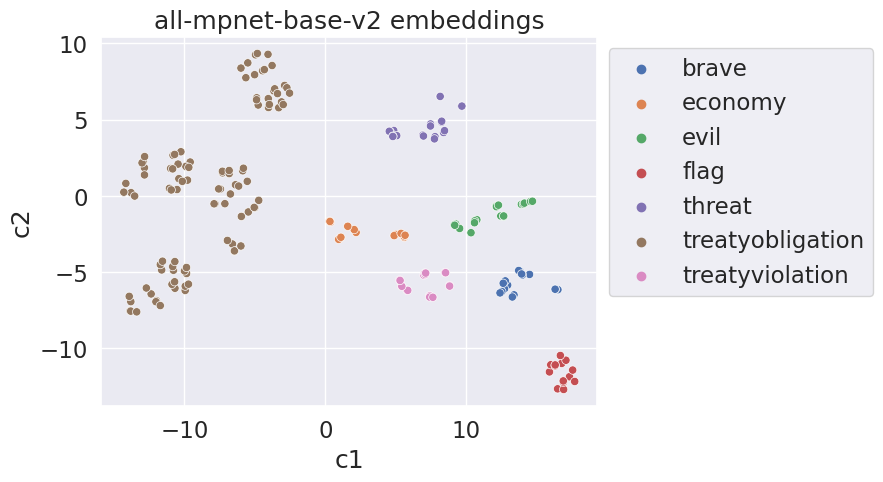
\includegraphics[width=0.45\textwidth]{plots/sanity_check/all-mpnet-base-v2.png}
    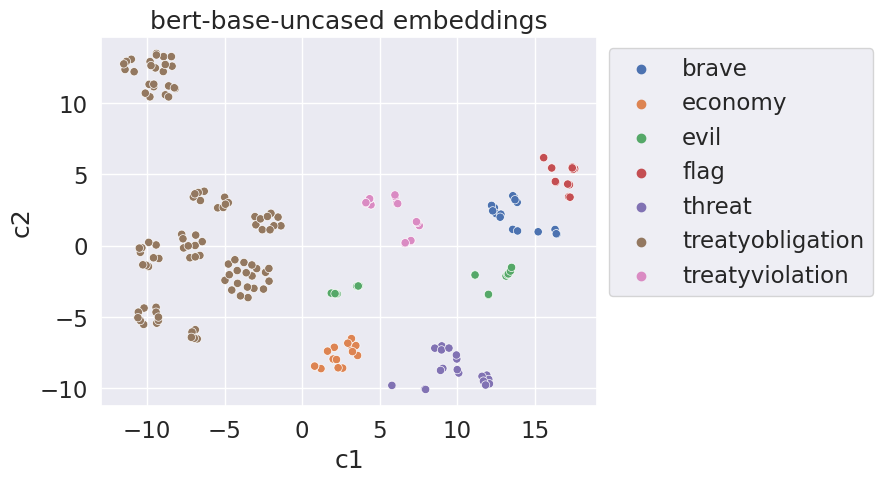
\includegraphics[width=0.45\textwidth]{plots/sanity_check/bert-base-uncased.png}
    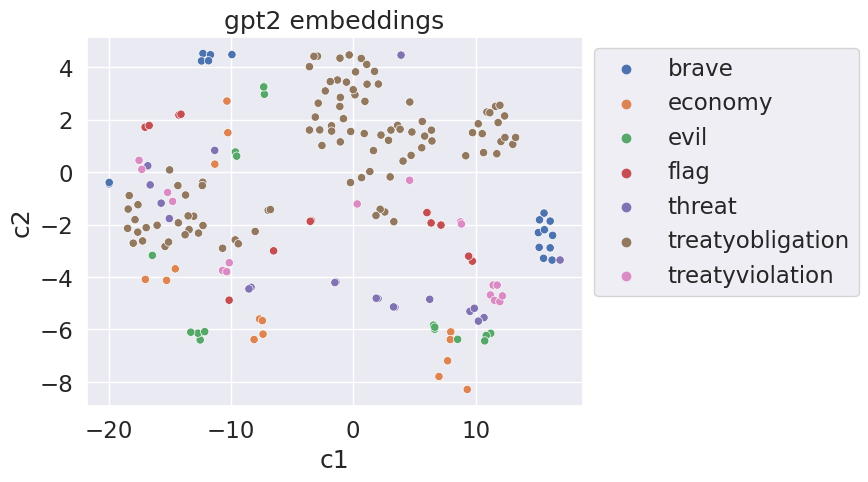
\includegraphics[width=0.45\textwidth]{plots/sanity_check/gpt2.png}
    \caption{t-SNE plots of sentence embeddings color-coded by the associated text attribute.}
    \label{fig:alias_check}
\end{figure}

We construct t-SNE plots of MPNet, BERT \cite{devlin2019bert}, and GPT-2 embeddings (Figure \ref{fig:alias_check}). Currently, we use MPNet embeddings in our classification approach and GPT-2 embeddings in our language modeling approach. While we see that MPNet and BERT embeddings separate clearly by text attribute (though some attributes--- \textit{commitment}/``treatyobligation'' and \textit{mistreatment}/``evil''---seem to form multiple clusters), GPT-2 clusters are less well-formed. This suggests that although GPT-2 produces effect estimates that seem empirically reasonable, we may want to use a different autoregressive language model that has more well-defined clusters. \vl{Or does it really matter, since we're not using GPT-2 language representations, only using it to estimate probabilities?}

\begin{figure}
    \centering
    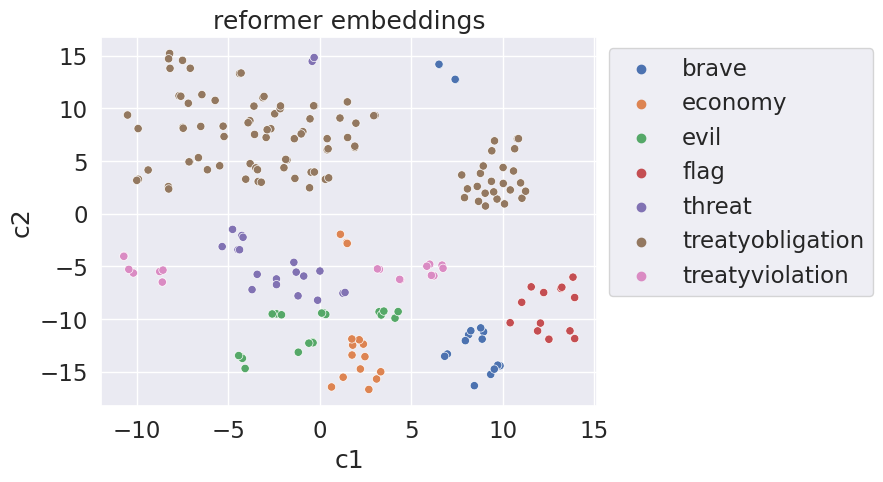
\includegraphics[width=0.45\textwidth]{plots/sanity_check/reformer.png}
    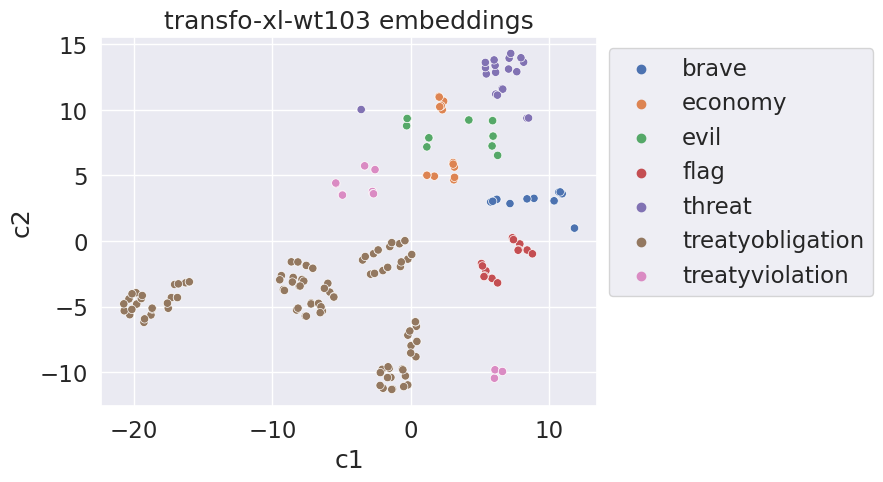
\includegraphics[width=0.45\textwidth]{plots/sanity_check/transfo-xl-wt103.png}
    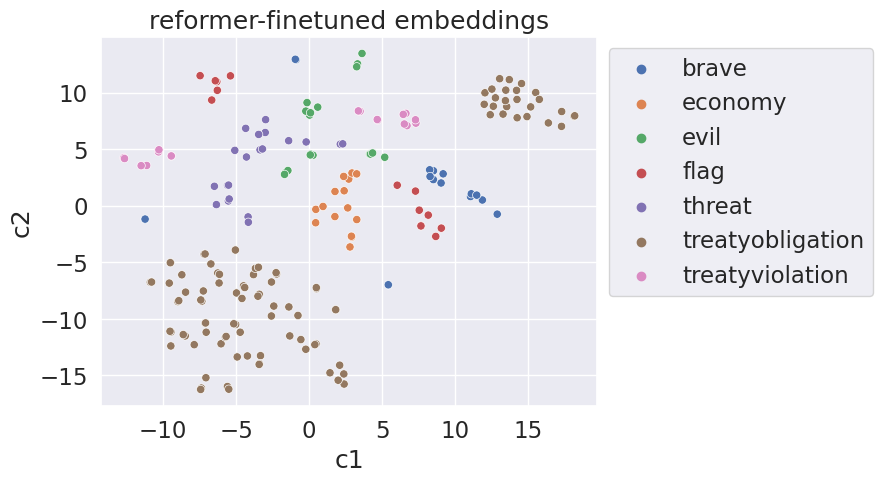
\includegraphics[width=0.45\textwidth]{plots/sanity_check/reformer-finetuned.png}
    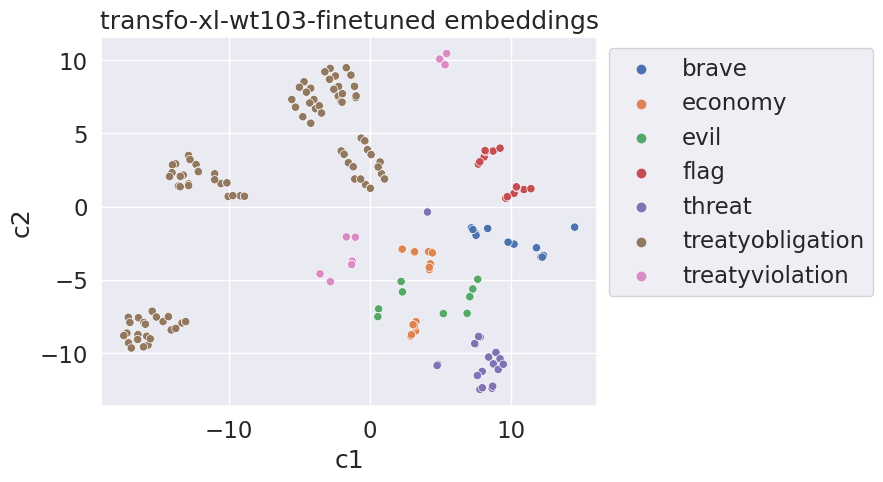
\includegraphics[width=0.45\textwidth]{plots/sanity_check/transfo-xl-wt103-finetuned.png}
    \caption{t-SNE plots of sentence embeddings color-coded by the associated text attribute.}
    \label{fig:alias_check2}
\end{figure}

\begin{table}[!ht]
    \centering
    \begin{tabular}{c|cccc}
        \toprule
        Treatment & $\hat{\mu}(P_1)$ & $\hat{\mu}(P_0)$ & $\hat{\tau}$ & 95\% CI \\
        \midrule
        Commitment & 71.242 & 68.785 & \textbf{\textcolor{green!50!black}{2.457$^*$}} & [0.024, 4.891] \\
        Bravery & 71.509 & 69.707 & \textcolor{green!50!black}{1.802} & [-1.004, 4.608] \\
        Mistreatment & 70.352 & 70.032 & \textcolor{green!50!black}{0.320} & [-2.516, 3.155] \\
        Flags & 68.436 & 70.544 & \textcolor{red!80!black}{-2.108} & [-5.121, 0.906] \\
        Threat & 68.697 & 70.517 & \textcolor{red!80!black}{-1.820} & [-4.626, 0.986]  \\
        Economy & 68.597 & 70.547 & \textcolor{red!80!black}{-1.950} & [-4.782, 0.882] \\
        Violation & 70.369 & 69.985 & \textcolor{green!50!black}{0.384} & [-2.515, 3.282] \\
        \bottomrule
    \end{tabular}
    \caption{Treatment effect estimates using the language modeling approach, where text probabilities under $P^T$ are estimated from Reformer fine-tuned with a CLM task on a small number of held-out samples from $P^T$.}
    \label{tab:results_clm_reformer}
\end{table}

\begin{table}[!ht]
    \centering
    \begin{tabular}{c|cccc}
        \toprule
        Treatment & $\hat{\mu}(P_1)$ & $\hat{\mu}(P_0)$ & $\hat{\tau}$ & 95\% CI \\
        \midrule
        Commitment & 70.779 & 68.715 & \textcolor{green!50!black}{2.064} & [-0.467, 4.596] \\
        Bravery & 71.041 & 69.275 & \textcolor{green!50!black}{1.766} & [-1.122, 4.654] \\
        Mistreatment & 70.174 & 69.62 & \textcolor{green!50!black}{0.554} & [-2.374, 3.482] \\
        Flags & 68.226 & 70.275 & \textcolor{red!80!black}{-2.049} & [-5.085, 0.987] \\
        Threat & 68.883 & 70.148 & \textcolor{red!80!black}{-1.265} & [-4.099, 1.568]  \\
        Economy & 69.332 & 70.005 & \textcolor{red!80!black}{-0.673} & [-3.509, 2.163] \\
        Violation & 70.166 & 69.63 & \textcolor{green!50!black}{0.536} & [-2.381, 3.453] \\
        \bottomrule
    \end{tabular}
    \caption{Treatment effect estimates using the language modeling approach, where text probabilities under $P^T$ are estimated from TransformerXL fine-tuned with a CLM task on a small number of held-out samples from $P^T$.}
    \label{tab:results_clm_transformerxl}
\end{table}

t-SNE plots of Reformer \cite{kitaev2020reformer} and TransformerXL \cite{dai2019transformerxl} (Figure \ref{fig:alias_check2}) show better separation by text attribute. We report additional results from the language modeling approach using these models to estimate text probabilities in Tables \ref{tab:results_clm_reformer} and \ref{tab:results_clm_transformerxl}. These estimates are somewhat more conservative that the ones produced by GPT-2 (in that only \textit{commitment} has a significant effect, and even then only for Reformer), and the effect directions are now consistent with the original study. 

\newpage
\appendix

\section{Extra notes}

\vl{These two subsections were generated using ChatGPT and are mostly for my own reference.}

\subsection{Change of measure with Radon-Nikodym derivatives}
\label{sec:change_of_measure}

The Radon-Nikodym derivative can be used to express one probability density function in terms of another probability density function, when the two densities are related by a change of measure. Specifically, if we have two probability measures defined on the same sample space, with one measure $\mathbb{P}$ absolutely continuous with respect to another measure $\mathbb{Q}$, then there exists a Radon-Nikodym derivative $Z$ such that:

$$\mathbb{P}(A) = \int_A Z d\mathbb{Q}$$

for any event $A$ in the sample space. Intuitively, this means that we can define the probability of any event under the measure $\mathbb{P}$ in terms of the probability of the same event under the measure $\mathbb{Q}$, by weighting the probabilities by a factor given by the Radon-Nikodym derivative.

Now, suppose we have two probability density functions $p(x)$ and $q(x)$ defined on some real-valued random variable $X$, with $q(x)>0$ for all $x$. We can interpret $q(x)$ as the "reference" density, and we want to express $p(x)$ in terms of $q(x)$ by a change of measure. To do this, we can define a new probability measure $\mathbb{P}$ as:
$$\mathbb{P}(A) = \int_A \frac{p(x)}{q(x)} q(x) dx = \int_A p(x) dx$$

for any event $A$ in the sample space. This means that we are weighting the probability of each event in proportion to the ratio $p(x)/q(x)$, which is a function of $x$. We can show that $\mathbb{P}$ is absolutely continuous with respect to the measure defined by $q(x)$, and therefore there exists a Radon-Nikodym derivative $Z(x)$ such that:
$$\frac{d\mathbb{P}}{d\mathbb{Q}}(x) = Z(x) = \frac{p(x)}{q(x)}$$

This means that we can express $p(x)$ in terms of $q(x)$ and the Radon-Nikodym derivative $Z(x)$, as:
$$p(x) = Z(x) q(x)$$

This is a general formula for expressing one probability density function in terms of another probability density function by a change of measure.

\subsection{Sentence probabilities from deep language models}
\label{sec:huggingface_sentence_probs}

To get the probability of a sentence from a HuggingFace transformers model, you first need to convert the sentence into a format that the model can understand. Typically, this involves tokenizing the sentence into a sequence of subwords, which is done using the tokenizer that corresponds to the pre-trained model you are using.

Once you have tokenized the sentence, you can pass it to the model to get the probability distribution over the possible output tokens. The probability of the sentence can be computed as the product of the probabilities of each individual token in the sequence.

Here's an example of how to get the probability of a sentence using the HuggingFace Transformers library in Python:

\begin{verbatim}
    from transformers import pipeline, AutoTokenizer, AutoModelForMaskedLM
    import torch
    
    # Load the pre-trained model and tokenizer
    model_name = "distilbert-base-uncased"
    tokenizer = AutoTokenizer.from_pretrained(model_name)
    model = AutoModelForMaskedLM.from_pretrained(model_name)
    
    # Define the input sentence
    input_sentence = "The cat sat on the mat."
    
    # Tokenize the input sentence
    tokens = tokenizer.encode(input_sentence, return_tensors="pt")
    
    # Get the probability distribution over the tokens
    outputs = model(tokens)
    predictions = torch.nn.functional.softmax(outputs.logits, dim=-1)
    
    # Compute the probability of the sentence
    probability = 1.0
    for i in range(1, len(tokens[0])):
    probability *= predictions[0, i, tokens[0, i]].item()
    
    print("The probability of the sentence is:", probability)
\end{verbatim}

This code uses the AutoTokenizer and AutoModelForMaskedLM classes from the Transformers library to load a pre-trained model and tokenizer. It then tokenizes the input sentence using the tokenizer, passes the resulting tokens to the model, and computes the probability of the sentence by multiplying together the probabilities of the individual tokens.

\section{Old results}

These results use the old randomization corpus generation method, which did not fully reflect the text generation method used by \cite{fong2021causal}. Additionally, data from the initial study by \cite{fong2021causal} is used, while the current results in the main body of the paper use the results from the replication study.

\begin{table}[!ht]
    \centering
    \begin{tabular}{c|cccc}
        \toprule
        Treatment & $\hat{\mu}(P_1)$ & $\hat{\mu}(P_0)$ & $\hat{\tau}$ & 95\% CI \\
        \midrule
        Commitment & 69.528 & 67.087 & \textcolor{green!50!black}{2.441} & [-7.458, 12.340] \\
        Bravery & 68.384 & 69.487 & \textcolor{red!80!black}{-1.103} & [-12.662, 10.457] \\
        Mistreatment & 69.570 & 68.757 & \textcolor{green!50!black}{0.813} & [-7.262, 8.887] \\
        Flags & 67.572 & 69.264 & \textcolor{red!80!black}{-1.692} & [-11.533, -8.149] \\
        Threat & 67.530 & 69.428 & \textcolor{red!80!black}{-1.898} & [-11.716, -7.922] \\
        Economy & 65.507 & 69.419 & \textcolor{red!80!black}{-3.912} & [-14.135, 6.312] \\
        Violation & 66.729 & 69.255 & \textcolor{red!80!black}{-2.526} & [-11.122, 6.070] \\
        \bottomrule
    \end{tabular}
    \caption{Treatment effect estimates using the classification approach, where the classifier is a logistic regression model learned over embeddings from pre-trained MPNet.}
    \label{tab:results_clf1_old}
\end{table}

\begin{table}[!ht]
    \centering
    \begin{tabular}{c|cccc}
        \toprule
        Treatment & $\hat{\mu}(P_1)$ & $\hat{\mu}(P_0)$ & $\hat{\tau}$ & 95\% CI \\
        \midrule
        Commitment & 64.695 & 65.918 & \textcolor{red!80!black}{-1.223} & [-21.573, 19.127] \\
        Bravery & 63.209 & 68.903 & \textcolor{red!80!black}{-5.694} & [-20.076, 8.688] \\
        Mistreatment & 67.990 & 65.089 & \textcolor{green!50!black}{2.902} & [-9.678, 15.582] \\
        Flags & 60.705 & 68.441 & \textcolor{red!80!black}{-7.737} & [-26.754, 11.280] \\
        Threat & 74.155 & 60.394 & \textcolor{green!50!black}{13.761} & [-4.433, 31.954] \\
        Economy & 59.555 & 65.373 & \textcolor{red!80!black}{-5.818} & [-22.012, 10.376] \\
        Violation & 65.028 & 65.210 & \textcolor{red!80!black}{-0.182} & [-12.003, 11.638] \\
        \bottomrule
    \end{tabular}
    \caption{Treatment effect estimates using the classification approach, where the classifier is a logistic regression model learned over embeddings from pre-trained MPNet. Text probabilities are computed from marginal sentence probabilities.}
    \label{tab:results_clf2_old}
\end{table}

\begin{table}[!ht]
    \centering
    \begin{tabular}{c|cccc}
        \toprule
        Treatment & $\hat{\mu}(P_1)$ & $\hat{\mu}(P_0)$ & $\hat{\tau}$ & 95\% CI \\
        \midrule
        Commitment & 68.377 & 62.907 & \textbf{\textcolor{green!50!black}{5.470}} & [1.944, 8.997] \\
        Bravery & 65.959 & 67.397 & \textcolor{red!80!black}{-1.439} & [-4.621, 1.744] \\
        Mistreatment & 68.266 & 66.625 & \textcolor{green!50!black}{1.641} & [-1.622, 4.904] \\
        Flags & 66.280 & 67.269 & \textcolor{red!80!black}{-0.990} & [-4.175, 2.196] \\
        Threat & 65.864 & 67.397 & \textcolor{red!80!black}{-1.532} & [-4.666, 1.602] \\
        Economy & 66.477 & 67.166 & \textcolor{red!80!black}{-0.689} & [-4.026, 2.649] \\
        Violation & 65.902 & 67.332 & \textcolor{red!80!black}{-1.429} & [-4.691, 1.832] \\
        \bottomrule
    \end{tabular}
    \caption{Treatment effect estimates using the language modeling approach, where text probabilities under $P^T$ are estimated from GPT-2 fine-tuned with a CLM task on a small number of held-out samples from $P^T$.}
    \label{tab:results_lm2_old}
\end{table}

\begin{table}[!ht]
    \centering
    \begin{tabular}{c|cccc}
        \toprule
        Treatment & $\hat{\mu}(P_1)$ & $\hat{\mu}(P_0)$ & $\hat{\tau}$ & 95\% CI \\
        \midrule
        Commitment & 67.694 & 61.536 & \textbf{\textcolor{green!50!black}{6.158}} & [2.212, 10.104] \\
        Bravery & 68.143 & 66.240 & \textcolor{green!50!black}{1.903} & [-1.380, 5.186] \\
        Mistreatment & 67.370 & 66.621 & \textcolor{green!50!black}{0.749} & [-2.642, 4.139] \\
        Flags & 66.935 & 66.812 & \textcolor{green!50!black}{0.123} & [-3.065, 3.311] \\
        Threat & 65.115 & 67.854 & \textcolor{red!80!black}{-2.739} & [-6.073, 0.595] \\
        Economy & 67.197 & 66.742 & \textcolor{green!50!black}{0.455} & [-2.895, 3.806] \\
        Violation & 66.283 & 67.180 & \textcolor{red!80!black}{-0.898} & [-4.169, 2.374] \\
        \bottomrule
    \end{tabular}
    \caption{Treatment effect estimates using the language modeling approach, where text probabilities under $P^T$ are estimated from pre-trained GPT-2. Text probabilities are computed from marginal sentence probabilities.}
    \label{tab:results_lm3_old}
\end{table}

\begin{table}[!ht]
    \centering
    \begin{tabular}{c|cccc}
        \toprule
        Treatment & $\hat{\mu}(P_1)$ & $\hat{\mu}(P_0)$ & $\hat{\tau}$ & 95\% CI \\
        \midrule
        Commitment & 69.254 & 66.250 & \textcolor{green!50!black}{3.004} & [-9.578, 15.586] \\
        Bravery & 68.617 & 68.317 & \textcolor{green!50!black}{0.301} & [-10.940, 11.542] \\
        Mistreatment & 71.439 & 67.742 & \textcolor{green!50!black}{3.696} & [-7.712, 15.103] \\
        Flags & 63.838 & 68.898 & \textcolor{red!80!black}{-5.060} & [-19.985, 9.865] \\
        Threat & 67.750 & 68.870 & \textcolor{red!80!black}{-1.120} & [-12.762, 10.522] \\
        Economy & 64.351 & 69.499 & \textcolor{red!80!black}{-5.148} & [-22.397, 12.101] \\
        Violation & 69.236 & 68.102 & \textcolor{green!50!black}{1.134} & [-10.067, 12.336] \\
        \bottomrule
    \end{tabular}
    \caption{Treatment effect estimates using the language modeling approach, where text probabilities under $P^T$ are estimated from pre-trained BERT. \vl{This is an improper approach since models trained with MLM, e.g. BERT, can't be used to estimate sentence probabilities directly.}}
    \label{tab:results_lm1_bert}
\end{table}

\newpage
\bibliographystyle{plain}
\bibliography{ref}

\end{document}